\documentclass[10pt]{article}

\input{joe/joe_notes_preamble.tex}
\usepackage{joe/bandit_macros}
\usepackage{joe/joe_macros}

\pagestyle{fancy}
\fancyhf{}
\rhead{}
\lhead{}
\rfoot{Page \thepage}

% title
\title{Mapping Class Group Orbits of Closed Curves on the Punctured Torus: Computed Counts and Tests of Conjectures}
\author{}
\date{}


\begin{document}
\maketitle
\tableofcontents

\section{Setup and Conventions}

\subsection{Curves, Words, Orbits}

Let $T$ be the once-punctured torus, with $\pi_1(T) \cong F(a,b)$ free on two generators and $A := a^{-1}$, $B := b^{-1}$.
Free homotopy classes of oriented closed curves on $T$ are conjugacy classes of $F(a,b)$, i.e.\ cyclically reduced words up to rotation (\emph{cyclic words}).
The puncture is the class of $\ttt{abAB}$.

\begin{defn}[Self-Intersection Number]
	For a free homotopy class $w$, $\operatorname{SI}(w)$ is the least number of transverse double points among general-position curves in the class.
\end{defn}

\begin{defn}[Orbit]
	By Dehn-Nielsen-Baer, the extended mapping class group of $T$ (all homeomorphisms up to isotopy, orientation-reversing included) is $\operatorname{Out}(F(a,b)) \cong \GL_2(\mb{Z})$.
	An \emph{orbit} is an orbit of this group on the set of \emph{unoriented} classes, so $w$ and $w^{-1}$ are the same curve.
	Let $N(k)$ be the number of orbits with $\operatorname{SI} = k$.
\end{defn}

\begin{defn}[Primitive]
	A class is \emph{primitive} if it is not a proper power $v^n$, $n \geq 2$.
	This is not the free-group sense of belonging to a basis.
	Let $N_{\text{prim}}(k)$ be the number of primitive orbits with $\operatorname{SI} = k$.
\end{defn}

\begin{fact}[Powers]
	For $v$ primitive and $n \geq 1$,
	\[
		\operatorname{SI}(v^n) = n^2 \operatorname{SI}(v) + n - 1 \, .
	\]
	Hence the non-primitive orbits at level $k$ are determined by the primitive orbits at lower levels.
	For $k = 4$ they are $a^5$ and $(\ttt{abAB})^5$; for $k = 5$ they are $a^6$, $(\ttt{abAB})^6$, $(\ttt{aabAB})^2$, $(\ttt{abaB})^2$.
\end{fact}

\begin{rmk}[other conventions]
	Three variants were also computed: oriented curves; orientation-preserving mapping classes only (the index-two subgroup of determinant $+1$); both.
	The counts differ from $k = 3$ on, since some classes are not equivalent to their inverse, resp.\ mirror image.
	See \Cref{tab:conventions}.
\end{rmk}

\section{Algorithms}

All code is in \ttt{src/}.
The original Java pipeline is in \ttt{old/}.

\subsection{Self-Intersection Number}

\begin{prop}[Linked Pairs]
	Embed the Cayley tree of $F(a,b)$ in the universal cover of $T$, with the four edges at each vertex in counterclockwise order $a, b, A, B$.
	The lifts of a primitive class $w$ are the axes of its conjugates.
	Two axes cross iff they meet in a (possibly degenerate) segment and arrive at it on opposite sides from how they leave it.
	Then $\operatorname{SI}(w)$ is the number of crossing pairs of axes up to the action of $F(a,b)$.
\end{prop}

\paragraph*{Implementation.}
For each pair of positions $(i,j)$ in the cyclic word, and each of the two relative orientations, walk along the common segment starting at the base vertex and compare the cyclic order of the incoming and outgoing letters.
Each unordered pair of axes is found twice.
Cost is $O(L^2)$ walks for a word of length $L$.
This is \ttt{freegroup.self\_intersection}; the same idea with two words gives \ttt{freegroup.intersection}.

\subsection{Orbits via Whitehead's Algorithm}

\begin{thm}[Whitehead, peak reduction]
	Let $W$ be the finite set of Whitehead automorphisms of $F(a,b)$.
	\begin{enumerate}[(a)]
		\item If a cyclic word is not of least length in its $\Aut$-orbit, some element of $W$ strictly shortens it.
		\item Two least-length cyclic words in the same orbit are joined by a chain of elements of $W$ passing only through least-length words.
		\item More generally every word of the orbit is reached from a least-length word by a chain along which length never decreases.
	\end{enumerate}
\end{thm}

A cyclic word of least length in its orbit is called \emph{minimal}.
The \emph{minimal set} of an orbit is its finite set of minimal words.

\begin{algo}[Canonical orbit representative]
	Shorten $w$ greedily to a minimal word, search the minimal set breadth-first under $W$ (adding $w \mapsto w^{-1}$ for unoriented curves), and return its lexicographically least element.
	Tracking the determinant along the search gives the orbit under orientation-preserving classes only.
\end{algo}

\subsection{Exhaustive Search}

\begin{prop}[Length Bound]\label{prop:length}
	Every orbit with $\operatorname{SI} = k$ contains a word of length $\leq 4(k+1)$.
\end{prop}

\begin{proof}
	By the basepoint lemma of \citet{crisp98}, a curve with $k$ self-intersections is freely homotopic to a product of $k+1$ simple loops meeting only at one point.
	By the loop classification of \citet{bck95}, in a suitable basis each of these is one of $a$, $b$, $ab$, $abA$, $baB$ or a rotation of $\ttt{abAB}$.
	Each has length $\leq 4$.
\end{proof}

\begin{lem}[Forced Crossings]
	Whether two lifts cross is decided by the letters along their common segment and one further letter at each end.
	For a linear word $x$ let $f(x)$ be the number of crossing pairs of lifts decided inside $x$.
	Then $f$ is non-decreasing along prefixes, and $f(x) \leq \operatorname{SI}(w)$ for every cyclic word $w$ containing $x$.
\end{lem}

\begin{algo}[\ttt{bruteforce.py}]
	Depth-first search over prefixes of cyclic words in canonical rotation (prenecklaces), of length $\leq 4(k+1)$, abandoning a prefix once $f > k$.
	Keep the minimal words with $\operatorname{SI} = k$ and sort them into orbits.
	By \Cref{prop:length} this finds every orbit.
\end{algo}

\begin{rmk}
	The search uses neither hand-drawn basepoint diagrams, nor loop arrangements, nor the unproven claim that one basepoint diagram suffices for $k = 4$.
	Running it to lengths $22, 24, 26$ for $k = 2, 3, 4$ finds no orbit beyond those of \Cref{prop:length}.
\end{rmk}

\subsection{Checks}

\begin{itemize}
	\item \ttt{self\_intersection} agrees with the Java library of Chas on $29{,}518$ words: every class of length $\leq 10$, and $20{,}000$ random words of length $\leq 40$.
	\item Orbit representatives are invariant under random automorphisms and inversion.
	\item The pruned search equals a naive enumeration of all words of length $\leq 11$, for $k \leq 4$.
	\item $N_{\text{prim}}(k) = 2, 2, 6, 14$ for $k = 0,\ldots,3$ agrees with \citet{crisp98,chas16}, and the $14$ orbits at $k=3$ are exactly those of Table 2 of \citet{chas16}.
	\item Minimal-position drawings (\ttt{draw.py}, geodesics on a one-holed torus) have exactly $\operatorname{SI}(w)$ crossings for every orbit with $k \leq 5$ and $300$ random words.
\end{itemize}

\section{Orbit Counts}

\subsection{Main Table}

\begin{table}[H]
	\centering
	\begin{tabular}{r|rr|rrr}
		\toprule
		$k$ & $N(k)$ & $N_{\text{prim}}(k)$ & annular & pants & filling \\
		\midrule
		0 & 2 & 2 & 2 & 0 & 0 \\
		1 & 4 & 2 & 2 & 2 & 0 \\
		2 & 8 & 6 & 2 & 5 & 1 \\
		3 & 16 & 14 & 2 & 11 & 3 \\
		4 & 29 & 27 & 2 & 18 & 9 \\
		5 & 57 & 53 & 2 & 34 & 21 \\
		6 & 109 & 107 & 2 & 60 & 47 \\
		7 & 204 & 202 & 2 & 110 & 92 \\
		8 & 369 & 367 & 2 & 181 & 186 \\
		9 & 669 & 661 & 2 & 306 & 361 \\
		10 & 1179 & 1177 & 2 & 502 & 675 \\
		\bottomrule
	\end{tabular}
	\caption{Orbits of unoriented curves under all homeomorphisms, by exhaustive search. The last three columns split $N(k)$ as in \Cref{sec:split}.}
	\label{tab:main}
\end{table}

\begin{table}[H]
	\centering
	\begin{tabular}{r|rrrr}
		\toprule
		$k$ & unoriented, all & oriented, all & unoriented, or.-pres. & oriented, or.-pres. \\
		\midrule
		0 & 2 & 2 & 2 & 3 \\
		1 & 4 & 4 & 4 & 6 \\
		2 & 8 & 8 & 8 & 14 \\
		3 & 16 & 17 & 17 & 30 \\
		4 & 29 & 35 & 35 & 66 \\
		5 & 57 & 73 & 74 & 139 \\
		6 & 109 & 149 & 152 & 292 \\
		7 & 204 & 309 & 310 & 604 \\
		8 & 369 & 596 & 603 & 1183 \\
		9 & 669 & 1127 & 1134 & 2235 \\
		10 & 1179 & 2058 & 2074 & 4102 \\
		\bottomrule
	\end{tabular}
	\caption{The same count under the four conventions (powers included).}
	\label{tab:conventions}
\end{table}

\begin{rmk}
	At $k = 3$ exactly one orbit, that of $\ttt{aabAbaBAb}$, is not equivalent to its inverse.
	At $k = 4$ there are six.
	\com{possibly the source of the count $15$ in \citet{bck95}; not checked against their list}
\end{rmk}

\begin{rmk}[OEIS]
	None of the sequences in \Cref{tab:main,tab:conventions}, their partial sums, or their first differences appears in the OEIS, even restricted to runs of five consecutive terms.
	None satisfies a linear recurrence of order $\leq 4$.
	No orbit counts for $k \geq 4$ were found in the literature.
\end{rmk}

\subsection{The Case $k = 4$}

The $29$ orbits, one shortest word each:
\begin{center}
	\ttt{aaaaa, aaabbb, aabbaB, aaaaabb, aaaabaB, aaabaaB, aaaaabAB, aaaabAAB, aaabAAAB, aabaBAbb,} \\
	\ttt{aaabABBAb, aabaBAbAB, aaaabbaBAb, aaabaBabAB, aaabaBAbaB, aabaaBabAB, aabbABabAB,} \\
	\ttt{aabABabbAB, aaaabABabAB, aaabAABabAB, aabABabABBAb, aaabbaBAbaBAb, aabaBabABabAB,} \\
	\ttt{aabaBAbaBAbaB, aaabABabABabAB, aabAABabABabAB, aabbaBAbaBAbaBAb,} \\
	\ttt{aabABabABabABabAB, abABabABabABabABabAB}
\end{center}

\begin{figure}[H]
	\centering
	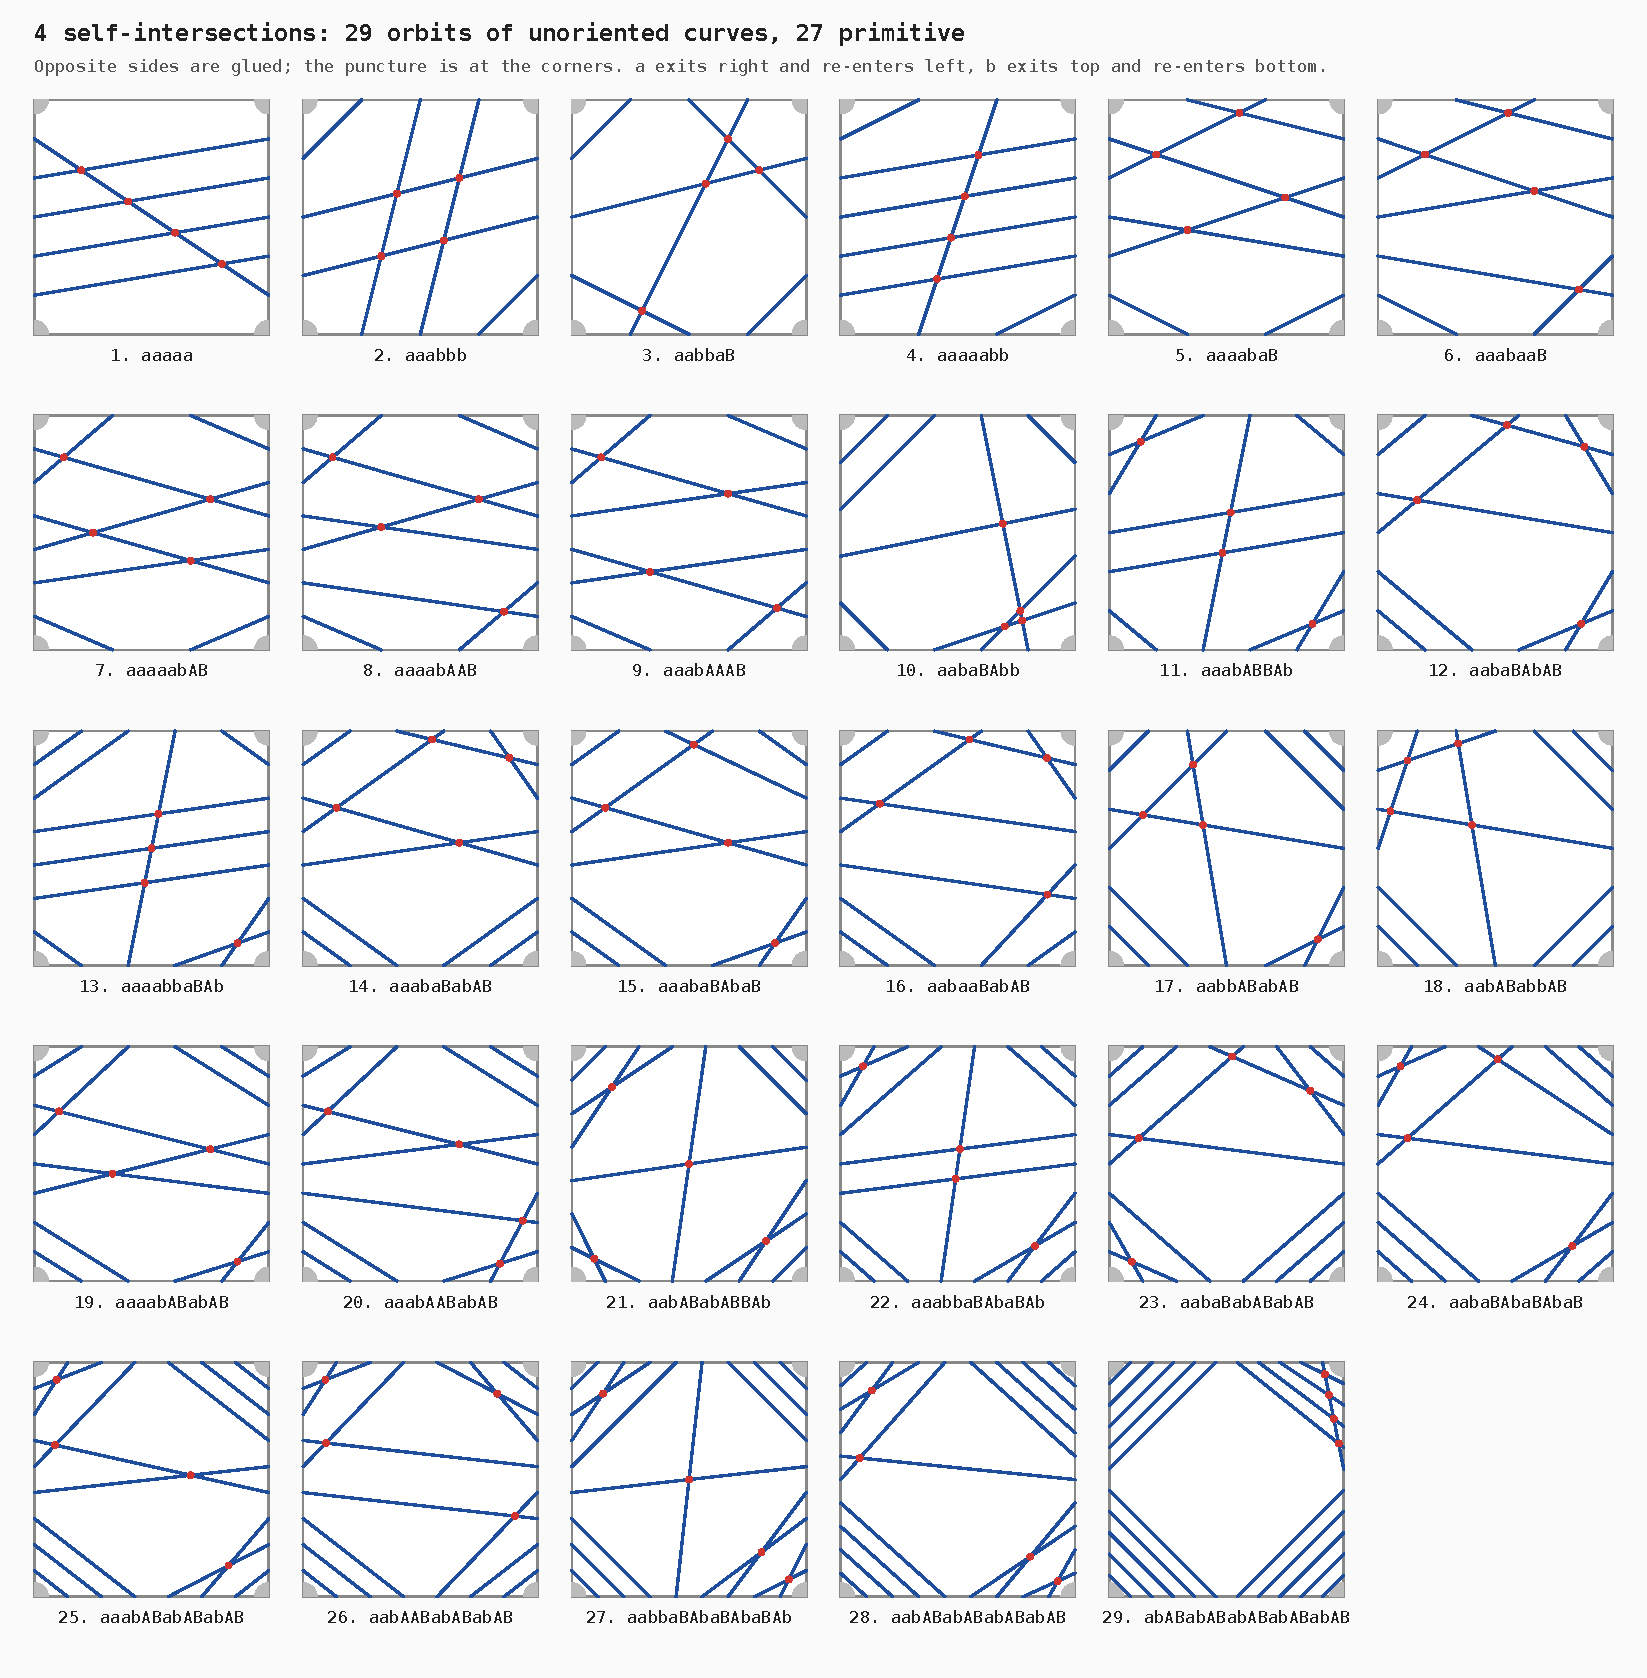
\includegraphics[width=0.9\textwidth]{../figures/k4.pdf}
	\caption{One curve from each orbit with four self-intersections, in minimal position. Opposite sides of each square are glued and the puncture is at the corners; $a$ exits right, $b$ exits top.}
\end{figure}

\paragraph*{Earlier claims.}
\begin{itemize}
	\item \ttt{Punctured Torus Count.tex} lists $44$ words; these contain only $28$ distinct orbits, and the orbit of \ttt{aabbaBAbaBAbaBAb} is missing.
	\item The Java output of $33$ words covers all $29$ orbits, counting four of them twice as a word and its inverse; as an oriented count the truth is $35$ and two are missing.
	\item The hand-made loop arrangements for $k = 3$ never produce the orbit of $\ttt{abaBAbAB}$; the Java total of $16$ matched the literature only because one orbit and its inverse were counted separately.
	\item The arrangement files contain a malformed ordering (nine entries), after which the Java reader silently drops the rest of the file, and four arrangements that produce curves with more than $k$ self-intersections, which no $k$-crossing picture can.
\end{itemize}

\section{Split by Filled Subsurface}\label{sec:split}

\begin{defn}
	A class is \emph{annular} if it is a power of a simple curve or of the puncture; \emph{pants} if it is not annular and is disjoint from some essential non-peripheral simple closed curve; \emph{filling} otherwise.
\end{defn}

\begin{lem}\label{lem:pants}
	\begin{enumerate}[(a)]
		\item A pants class is disjoint from exactly one simple closed curve $\alpha$, and lies in the pair of pants $T \setminus \alpha$.
		\item A class is disjoint from the simple curve $a$ iff it is conjugate into $\langle a, bAB \rangle$, iff the letters $b$, $B$ alternate around its cyclic word.
		\item Such an alternating word is minimal.
	\end{enumerate}
\end{lem}

\begin{proof}
	(a) Two distinct such curves fill $T$, so a class disjoint from both is peripheral.
	(b) $\pi_1(T \setminus a) = \langle a, bAB \rangle$.
	(c) Write the word as $x^{i_1} y^{j_1} \cdots x^{i_m} y^{j_m}$ with $x = a$, $y = bAB$.
	The Whitehead automorphisms multiplying $b$ by $a^{\pm 1}$ fix the cyclic word.
	Those multiplying $a$ by $b^{\pm 1}$ change its length by $\sum_r (|i_r| + |j_r|) - 2m \geq 0$.
\end{proof}

So an orbit is non-filling iff some word of its minimal set is alternating; this is \ttt{filling.py}.

\begin{rmk}[checks]
	For all $225$ orbits with $k \leq 6$, and all simple curves of word length $\leq 9$: pants orbits have zero intersection number with exactly one simple curve, filling orbits with none, powers of the puncture with all.
	Independently, enumerating words in the pants generators up to the length bound $2k+2$ of \citet{chasphillips12} and sorting into orbits reproduces the pants column for $k \leq 5$.
\end{rmk}

\begin{rmk}
	The pants column counts closed curves on a pair of pants with $k$ self-intersections up to the four symmetries fixing one boundary component.
	Filling orbits overtake pants orbits at $k = 8$; their step ratio is close to $2$ ($1.96, 2.02, 1.94, 1.87$ for $k = 7,\ldots,10$) against $1.83, 1.65, 1.69, 1.64$ for pants.
\end{rmk}

\section{Growth of $N(k)$}

\subsection{Known Bounds}

Let $O(K,S)$ be the number of orbits with $\operatorname{SI} \leq K$ on a surface $S$.

\begin{thm}[\citealt{sapir16}]
	For any compact $S$ and $K \geq 1$,
	\[
		\tfrac{1}{12}\, 2^{\sqrt{K/12}} \leq O(K,S) \leq \exp\bigl(d_S \sqrt{K} \log(d_S \sqrt{K})\bigr) \, .
	\]
	The lower bound comes from curves in an embedded pair of pants, whose stabilizer in the mapping class group is finite.
\end{thm}

\begin{thm}[\citealt{aougabsouto16}]
	For $S$ closed and every $\delta > 0$, for $K$ large,
	\[
		\exp\bigl((\pi\sqrt{|\chi(S)|} - \delta)\sqrt{K}\bigr) \leq O(K,S) \leq \exp\bigl((4\sqrt{2|\chi(S)|} + \delta)\sqrt{K}\bigr) \, .
	\]
	The upper bound holds for every finite-type orientable $S$ with $\chi(S) < 0$ (their Sec.\ 7.1).
	They conjecture that the lower bound is sharp.
\end{thm}

\begin{claim}[research note \ttt{curve\_orbit\_bounds.pdf}, not independently verified]
	For $S = T$ and $K$ large, the number of orbits with $\operatorname{SI}$ \emph{exactly} $K$ is at least $\frac{c}{\sqrt{K}}\, 3^{3\sqrt{K} - 9K^{1/4}}$, so that
	\[
		3\log(3) \leq \liminf_{K \to \infty} \frac{\log N(K)}{\sqrt{K}} \leq \limsup_{K \to \infty} \frac{\log N(K)}{\sqrt{K}} \leq 4\sqrt{2} \, .
	\]
	The construction takes a typical word of length $\approx 3\sqrt{K}$ in a pair of pants, where $\operatorname{SI} \approx N^2/9$ \citep{chaslalley12}, and pads its unique longest block.
\end{claim}

\begin{lem}[Padding, from the same note]
	In pants generators, if $a^M u$ is cyclically reduced, $u$ begins and ends with $b^{\pm 1}$, and every $a^{\pm 1}$-block of $u$ is shorter than $M$, then $\operatorname{SI}(a^{M+d} u) = \operatorname{SI}(a^M u) + d$ for all $d \geq 0$.
\end{lem}

\begin{rmk}[checks]
	The padding identity holds in $4{,}500$ random cases, and fails in $426$ of $1{,}500$ random cases when the unique-longest-block hypothesis is dropped.
	The transfer from pants to $T$ is the argument of \citet{sapir16}.
	The statement for exactly $K$, and the constant $3\log(3)$, were not found in \citet{sapir16,aougabsouto16}, which count $\operatorname{SI} \leq K$.
\end{rmk}

\com{$3\log(3) \approx 3.30 > \pi$, the value conjectured by Aougab-Souto at $|\chi| = 1$ (stated for closed $S$). Their intersection form may count each crossing twice, in which case their constant per crossing is $\pi\sqrt{2} \approx 4.44$ and there is no conflict. Convention not settled from their text.}

\subsection{Fits to the Data}

\begin{table}[H]
	\centering
	\begin{tabular}{r|rrrrrrrrrr}
		\toprule
		$k$ & 1 & 2 & 3 & 4 & 5 & 6 & 7 & 8 & 9 & 10 \\
		\midrule
		$N(k)/N(k-1)$ & 2 & 2 & 2 & 1.81 & 1.97 & 1.91 & 1.87 & 1.81 & 1.81 & 1.76 \\
		\bottomrule
	\end{tabular}
\end{table}

Least squares on $\log N(k)$, $k = 1,\ldots,8$:

\begin{table}[H]
	\centering
	\begin{tabular}{l|l|r|rr}
		\toprule
		model & fitted & rms error & predicted $N(9)$ & predicted $N(10)$ \\
		\midrule
		$\exp(c\sqrt{k})$ & $c = 2.5$ & $0.18$ & & \\
		$k^{-a}\exp(c\sqrt{k})$ & $c = 4.45$, $a = 1.76$ & $0.034$ & $\approx 627$ & $\approx 1070$ \\
		$\exp(\alpha k)$ & $e^{\alpha} = 1.91$ & $0.032$ & $\approx 736$ & $\approx 1400$ \\
		$k^{a}\exp(\alpha k)$ & $e^{\alpha} = 1.84$, $a = 0.14$ & $0.018$ & $\approx 700$ & $\approx 1310$ \\
		\midrule
		actual & & & $669$ & $1179$ \\
		\bottomrule
	\end{tabular}
\end{table}

\begin{rmk}
	\begin{itemize}
		\item Bare $\exp(c\sqrt{k})$ does not fit; a power-law prefactor is needed.
		\item With the prefactor, $c$ is unstable: $4.45$ on $k \in [1,8]$, $5.5$ on $k \in [3,8]$.
		\item The data for $k \leq 8$ do not separate $\exp(c\sqrt{k})$ from $\exp(\alpha k)$; the values at $k = 9, 10$ fall between the two predictions.
		\item The asymptotic regime is far away: the inequality used in the claim above needs $K^{1/4} \geq 6 + 3\sqrt{3}$, i.e.\ $K \gtrsim 1.5 \times 10^4$.
		\item At $k = 10$ the shortest words of the orbits have lengths $9$ to $44$ with mode $15$, against the typical-word length $3\sqrt{k} \approx 9.5$: the orbits seen are long words with unusually few crossings.
	\end{itemize}
\end{rmk}

\com{heuristic: the true constant should exceed $3\log(3)$. Words with slightly fewer crossings per length than typical are only second-order rarer in entropy, but gain first-order in length for the same $K$.}

\section{Chas's Conjectures on Orbit Sizes}

\subsection{Statements}

For an orbit $\alpha$ of unoriented curves let $c_\ell(\alpha)$ be the number of its classes of word length $\ell$, and let $\phi$ be Euler's function, extended by $0$ off the positive integers.

\begin{conj}[\citealt{chas16}, Conjecture 4]\label{conj:four}
	For every $\alpha$ there are integers $j_i$ and $k_i \geq 1$ with
	\[
		c_\ell(\alpha) = 2 \sum_{i=1}^n \phi\Bigl(\frac{\ell + j_i}{k_i}\Bigr)
	\]
	for $\ell$ large.
	Then $\sum_{\ell \leq L} c_\ell(\alpha) \sim \frac{6}{\pi^2}\, p_\alpha L^2$ with $p_\alpha := \sum_i k_i^{-2}$.
\end{conj}

\begin{conj}[\citealt{chas16}, Conjecture 5]\label{conj:five}
	For each $k$, the sum of $p_\alpha$ over the primitive non-peripheral orbits with $\operatorname{SI} = k$ is within $1$ of the number of such orbits.
\end{conj}

\subsection{Method}

By part (c) of Whitehead's theorem, a breadth-first search from the minimal set under $W$, discarding words longer than $L$, finds every class of the orbit of length $\leq L$.
This gives $c_\ell(\alpha)$ exactly for $\ell \leq L$ (\ttt{orbit\_growth.py}).
A formula of the shape of \Cref{conj:four} is then searched for, fewest terms first, with $k_i \leq 12$, shifts that are multiples of $4$ tried first.
Formulas are fitted on $\ell \leq 60$.

\subsection{Results}

\begin{table}[H]
	\centering
	\begin{tabular}{r|r|l|r}
		\toprule
		$k$ & orbits & $\sum_\alpha p_\alpha$ & difference \\
		\midrule
		0 & 1 & $1$ & $0$ \\
		1 & 2 & $9/4$ & $+0.25$ \\
		2 & 6 & $197/36 \approx 5.47$ & $-0.53$ \\
		3 & 14 & $2023/144 \approx 14.05$ & $+0.05$ \\
		4 & 27 & $\geq 103951/3600 \approx 28.88$; estimated $\approx 30.2$ & $\geq +1.88$; $\approx +3.2$ \\
		5 & 53 & $\geq 6691/120 \approx 55.76$; estimated $\approx 62.2$ & $\geq +2.76$; $\approx +9.2$ \\
		\bottomrule
	\end{tabular}
	\caption{Test of \Cref{conj:five}. For $k = 4, 5$ the lower bound is the exact sum over the orbits with a fitted formula ($25$ of $27$, resp.\ $47$ of $53$).}
\end{table}

\begin{claim}
	\Cref{conj:five} fails at $k = 4$ and $k = 5$, granting that the fitted formulas hold for all $\ell$.
\end{claim}

\begin{rmk}[evidence]
	\begin{itemize}
		\item For $k \leq 3$ the method recovers every formula of Tables 1 and 2 of \citet{chas16}, including those marked unproven.
		\item Every formula fitted on $\ell \leq 60$ predicts $c_\ell$ exactly for $61 \leq \ell \leq 84$: all $25$ at $k = 4$ and all $47$ at $k = 5$.
		\item For the orbits without a formula, $p_\alpha$ is estimated by a two-point extrapolation of $\sum_{\ell \leq L} c_\ell$ at $L = 60, 84$; on the fitted orbits this method gives $28.5$ against the exact $28.88$.
	\end{itemize}
\end{rmk}

\begin{rmk}
	Table 4 of \citet{chas16} gives $2059/144$ at $k = 3$; the entries of her Table 2 sum to $2023/144$, which is the value found here.
\end{rmk}

\begin{table}[H]
	\centering
	\small
	\begin{tabular}{l|l|r|r}
		\toprule
		orbit & $c_\ell$ & valid for $\ell \geq$ & $p_\alpha$ \\
		\midrule
		\ttt{aaabbb} & no formula found & & $\approx 0.65$ \\
		\ttt{aabbaB} & $4\phi(\ell-4) + 4\phi(\ell)$ & 7 & $4$ \\
		\ttt{aaaaabb} & no formula found & & $\approx 0.69$ \\
		\ttt{aaaabaB} & $4\phi(\ell/5)$ & 8 & $2/25$ \\
		\ttt{aaabaaB} & $4\phi(\ell/5)$ & 8 & $2/25$ \\
		\ttt{aaaaabAB} & $4\phi((\ell-4)/4)$ & 8 & $1/8$ \\
		\ttt{aaaabAAB} & $4\phi((\ell-4)/4)$ & 8 & $1/8$ \\
		\ttt{aaabAAAB} & $2\phi((\ell-4)/4)$ & 8 & $1/16$ \\
		\ttt{aabaBAbb} & $16\phi((\ell-4)/2)$ & 9 & $2$ \\
		\ttt{aaabABBAb} & $2\phi(\ell-8) + 2\phi(\ell-4)$ & 10 & $2$ \\
		\ttt{aabaBAbAB} & $8\phi((\ell-4)/3)$ & 10 & $4/9$ \\
		\ttt{aaaabbaBAb} & $8\phi((\ell-8)/2) + 8\phi((\ell-4)/2)$ & 11 & $2$ \\
		\ttt{aaabaBabAB} & $8\phi((\ell-4)/4)$ & 11 & $1/4$ \\
		\ttt{aaabaBAbaB} & $4\phi((\ell-4)/4)$ & 11 & $1/8$ \\
		\ttt{aabaaBabAB} & $8\phi((\ell-4)/4)$ & 11 & $1/4$ \\
		\ttt{aabbABabAB} & $8\phi(\ell-8)$ & 11 & $4$ \\
		\ttt{aabABabbAB} & $8\phi(\ell-8)$ & 11 & $4$ \\
		\ttt{aaaabABabAB} & $4\phi((\ell-8)/3)$ & 11 & $2/9$ \\
		\ttt{aaabAABabAB} & $8\phi((\ell-8)/3)$ & 11 & $4/9$ \\
		\ttt{aabABabABBAb} & $4\phi((\ell-8)/2)$ & 13 & $1/2$ \\
		\ttt{aaabbaBAbaBAb} & $4\phi(\ell-12) + 4\phi(\ell-8)$ & 14 & $4$ \\
		\ttt{aabaBabABabAB} & $8\phi((\ell-8)/3)$ & 14 & $4/9$ \\
		\ttt{aabaBAbaBAbaB} & $4\phi((\ell-8)/3)$ & 14 & $2/9$ \\
		\ttt{aaabABabABabAB} & $4\phi((\ell-12)/2)$ & 14 & $1/2$ \\
		\ttt{aabAABabABabAB} & $4\phi((\ell-12)/2)$ & 14 & $1/2$ \\
		\ttt{aabbaBAbaBAbaBAb} & $4\phi((\ell-12)/2)$ & 17 & $1/2$ \\
		\ttt{aabABabABabABabAB} & $4\phi(\ell-16)$ & 17 & $2$ \\
		\bottomrule
	\end{tabular}
	\caption{Orbit sizes for the $27$ primitive orbits with $k = 4$. The table for $k = 5$ is in \ttt{results/growth\_k5.txt}.}
\end{table}

\begin{rmk}[on \Cref{conj:four}]
	No formula was found for $a^3b^3$, $a^5b^2$ at $k = 4$ and for six orbits at $k = 5$ (\ttt{aaaaaabb}, \ttt{aaabbabb} and four with $p_\alpha \approx 1.33$).
	For $a^3 b^3$ the counts along $\ell \equiv 1 \pmod{6}$ are $4, 4, 4, 8, 12, 12, 16, 16, 20, 24, 24$ for $\ell = 7, 13, \ldots, 67$, which grows smoothly, unlike totient sums.
	The estimates $p \approx 0.65$ and $p \approx 1.33$ suggest $2/3$ and $4/3$, which are not sums of $k_i^{-2}$ in any evident way.
	\com{whether \Cref{conj:four} fails for these orbits is open; a wider search ($k_i \leq 12$, up to $16$ terms) timed out without a result}
\end{rmk}

\section{From Level $k-1$ to Level $k$}

\subsection{Smoothing a Crossing}

At a self-intersection the cyclic word splits as $w = uv$ into two loops based at the crossing.
The smoothing that keeps one component is $u v^{-1}$, with $\operatorname{SI}(u v^{-1}) \leq \operatorname{SI}(w) - 1$.
Conversely, if $p = \alpha\beta$ then every curve obtained from $p$ by adding one crossing is
\[
	\alpha\, \gamma^{-1} \beta^{-1} \gamma^{-1}
\]
for some word $\gamma$, the class of an arc joining the two points where $p$ is cut.

\begin{claim}[verified for $1 \leq k \leq 8$]\label{claim:parent}
	Every primitive orbit with $\operatorname{SI} = k$ has a crossing whose smoothing has $\operatorname{SI}$ exactly $k-1$.
	Every orbit with $\operatorname{SI} = k-1$, powers included, arises this way.
\end{claim}

\begin{rmk}
	The relation is many-to-many: at $k = 8$ an orbit has $1$ to $7$ distinct parents and a parent up to $18$ children; about $44\%$ of smoothings drop $\operatorname{SI}$ by exactly one.
	Generating level $k$ from minimal words of level $k-1$ with $|\gamma| \leq 2$ is incomplete: it finds $199$ of the $202$ primitive orbits at $k = 7$.
	An exact generator would need the arcs $\gamma$ inside faces of all minimal-position diagrams of the parent.
\end{rmk}

\subsection{Loop Insertion and the Stable Range}

A \emph{loop insertion} inserts one of the eight rotations of $(\ttt{abAB})^{\pm 1}$ into a minimal word at any position, keeping the result if it is cyclically reduced as written, minimal, and has one more self-intersection.

\begin{claim}[verified for $2 \leq k \leq 10$]\label{claim:loop}
	The orbits with $\operatorname{SI} = k$ whose minimal words have length $\geq 2k+3$ are exactly the loop insertions of the orbits with $\operatorname{SI} = k-1$ whose minimal words have length $\geq 2k-1$.
\end{claim}

\begin{table}[H]
	\centering
	\begin{tabular}{r|rrrrrrrrr}
		\toprule
		$k$ & 2 & 3 & 4 & 5 & 6 & 7 & 8 & 9 & 10 \\
		\midrule
		orbits of length $\geq 2k+3$ & 3 & 8 & 11 & 20 & 31 & 58 & 85 & 140 & 213 \\
		parents (level $k-1$, length $\geq 2k-1$) & 3 & 7 & 11 & 19 & 31 & 57 & 85 & 139 & 213 \\
		orbits that are not loop insertions & 4 & 7 & 11 & 22 & 41 & 66 & 112 & 191 & \\
		their greatest length & 6 & 8 & 9 & 12 & 14 & 16 & 17 & 20 & \\
		\bottomrule
	\end{tabular}
	\caption{Each parent has exactly one child, except one parent with two at each odd $k$. The last two rows use loop insertions from all of level $k-1$.}
\end{table}

\begin{rmk}
	The threshold $2k+2$ is sharp: at most levels some orbit that is not a loop insertion has minimal length exactly $2k+2$.
	In the stable range the number of orbits with minimal length $\ell$ at level $k$ equals the number with length $\ell - 4$ at level $k-1$ (for even $k$; at odd $k$ there is one more).
	Filling orbits have minimal length up to $4k-3$, pants orbits up to $4k+1$, the puncture power $4k+4$.
\end{rmk}

\begin{algo}[\ttt{fast.py}]
	For $k \geq 2$: exhaustive search to length $2k+2$, union the loop insertions of the level $k-1$ orbits of length $\geq 2k-1$.
	Every orbit reported is verified individually, so if \Cref{claim:loop} failed at some $k$ the count would be too small, never too large.
\end{algo}

\begin{table}[H]
	\centering
	\begin{tabular}{r|rrrrrrr}
		\toprule
		$k$ & 6 & 7 & 8 & 9 & 10 & 11 & 12 \\
		\midrule
		\ttt{bruteforce.py} (seconds, 16 cores) & 16 & 66 & 216 & & 1676 & & \\
		\ttt{fast.py} (seconds, 16 cores) & 1.2 & 2.5 & 6.0 & 15.9 & 48.8 & 113 & 268 \\
		\bottomrule
	\end{tabular}
	\caption{Running times. For $k \leq 10$ the two methods return identical sets of orbits.}
\end{table}

\begin{table}[H]
	\centering
	\begin{tabular}{r|rr|rrr|r}
		\toprule
		$k$ & $N(k)$ & $N_{\text{prim}}(k)$ & annular & pants & filling & $N(k)/N(k-1)$ \\
		\midrule
		11 & 2081 & 2077 & 2 & 840 & 1239 & 1.77 \\
		12 & 3602 & 3600 & 2 & 1359 & 2241 & 1.73 \\
		\bottomrule
	\end{tabular}
	\caption{Counts from \ttt{fast.py} beyond the range of the exhaustive search. These are exact if \Cref{claim:loop} holds at $k = 11, 12$, and lower bounds otherwise.}
\end{table}

\begin{rmk}
	The non-primitive counts agree with the power formula: $4$ at $k = 11$ ($a^{12}$, $(\ttt{abAB})^{12}$ and the cubes of the two primitive orbits with $k = 1$) and $2$ at $k = 12$.
\end{rmk}

\section{Open Questions}

\begin{enumerate}
	\item Prove \Cref{claim:loop}. A natural route: a minimal word of length $\geq 2k+3$ with $\operatorname{SI} = k$ must contain a loop round the puncture whose removal costs exactly one crossing, in analogy with the bound $L \leq 2k+2$ of \citet{chasphillips12} on the pair of pants.
	\item Prove \Cref{claim:parent}.
	\item Decide \Cref{conj:four} for $a^3 b^3$ and $a^5 b^2$; find $p_\alpha$ exactly for the orbits of $a^p b^q$.
	\item Is there a corrected form of \Cref{conj:five}? The excess $\sum_\alpha p_\alpha - N_{\text{prim}}(k)$ is $0, 0.25, -0.53, 0.05, \approx 3.2, \approx 9.2$.
	\item The constant in $\log N(k) \sim c\sqrt{k}$, and whether the limit exists; settle the counting convention in \citet{aougabsouto16}.
	\item A formula or recursion for the pants column, using the block structure of words in $\langle a, bAB\rangle$ and the intersection formula of \citet{diopgaye22}.
\end{enumerate}

\begin{thebibliography}{99}

\bibitem[Aougab and Souto(2016)]{aougabsouto16}
T. Aougab and J. Souto.
\newblock Counting curve types.
\newblock arXiv:1606.06067, 2016.

\bibitem[Butler et~al.(1995)]{bck95}
M. Butler, J. Carton, and E. Kraft.
\newblock Geodesics with three intersections on the punctured torus.
\newblock Proceedings of the REU Program in Mathematics, Oregon State University, 1995.

\bibitem[Chas(2016)]{chas16}
M. Chas.
\newblock Non-abelian number theory and the structure of curves on surfaces.
\newblock arXiv:1608.02846, 2016.

\bibitem[Chas and Lalley(2012)]{chaslalley12}
M. Chas and S. P. Lalley.
\newblock Self-intersections in combinatorial topology: statistical structure.
\newblock Invent.\ Math.\ 188:429--463, 2012.

\bibitem[Chas and Phillips(2012)]{chasphillips12}
M. Chas and A. Phillips.
\newblock Self-intersection numbers of curves in the doubly-punctured plane.
\newblock Exp.\ Math.\ 21(1):26--37, 2012.

\bibitem[Crisp et~al.(1998)]{crisp98}
D. Crisp, S. Dziadosz, D. Garity, T. Insel, T. Schmidt, and P. Wiles.
\newblock Closed curves and geodesics with two self-intersections on the punctured torus.
\newblock Monatsh.\ Math.\ 125:189--209, 1998.

\bibitem[Diop and Gaye(2022)]{diopgaye22}
E. H. A. A. Diop and M. Gaye.
\newblock Self intersections on a pair of pants.
\newblock arXiv:2108.06796, 2022.

\bibitem[Sapir(2016)]{sapir16}
J. Sapir.
\newblock Orbits of non-simple closed curves on a surface.
\newblock arXiv:1602.09093, 2016.

\end{thebibliography}

\end{document}
